\documentclass{article}

\usepackage{mathrsfs,amsmath}
\usepackage{xcolor}
\usepackage{titlesec}
\usepackage{listings}
\usepackage{syntax}
\usepackage{pythonhighlighting}
\usepackage{graphicx}

\graphicspath{ {./assets/} }

\usepackage[margin=1.4in]{geometry}

\title{Handout \#8 | CS 471} 
\author{Jared Dyreson\\ 
        California State University, Fullerton}

\DeclareRobustCommand{\bowtie}{%
  \mathrel\triangleright\joinrel\mathrel\triangleleft}


\usepackage [english]{babel}
\usepackage [autostyle, english = american]{csquotes}
\MakeOuterQuote{"}

\titlespacing*{\section}
{0pt}{5.5ex plus 1ex minus .2ex}{4.3ex plus .2ex}
\titlespacing*{\subsection}
{0pt}{5.5ex plus 1ex minus .2ex}{4.3ex plus .2ex}

\usepackage{hyperref}
\hypersetup{
    colorlinks,
    citecolor=black,
    filecolor=black,
    linkcolor=black,
    urlcolor=black
}

\begin{document}

\maketitle
\tableofcontents

\newpage

\section{Questions}

\begin{enumerate}
\item Give sample HTTP commands executed by the browser in order to download the page "index.html" from the server "ecs.fullerton.edu"
\begin{verbatim} 
GET /index.html HTTP/1.1

User Agent: Mozilla /5.0 (Compatible, Intel MAC OS X, Macintosh)

Host: www.ecs.fullerton.edu

Accept-Language: en-us

Accept-Encoding: gzip, deflate

Connection: keep-Alive
\end{verbatim}
\item Give a quantitative example illustrating the benefits of a web caching proxy
\begin{itemize}
\item CDNs perform proxy caching on a mass scale
\item More information can be read about \href{https://blog.stackpath.com/proxy-caching/}{\underline{here}}
\end{itemize}

\item Describe the basic structure of the HTTP request and response message
\begin{figure}[!h]
\centering
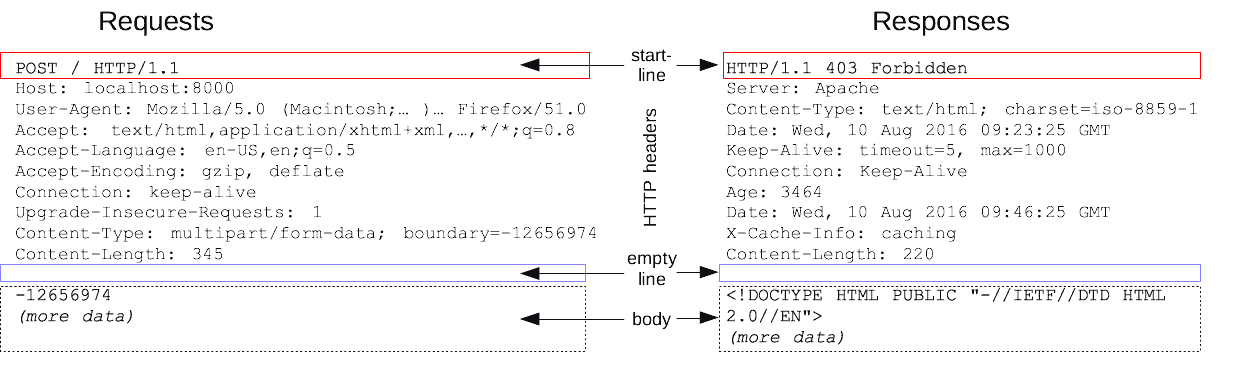
\includegraphics[width=10cm]{httpmsgstructure2}
\end{figure}
\item What is the conditional GET request?
\begin{itemize}
\item Different validators in the request header can produce different resources, such as region locked content or a specific version of a page (last modified).
\begin{figure}[!h]
\centering
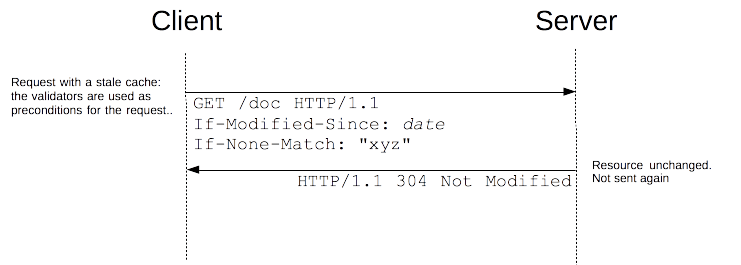
\includegraphics[width=10cm]{httpcache2}
\end{figure}
\end{itemize}
\newpage

\item Why does the HTTP response from the origin web server to the caching proxy server include only the message header if the object in question has not changed?
\begin{itemize}
\item The HTTP response is letting us know that it is using cached data in the form of status codes. 304 in particular tells us this. There is no reason to return information that is not different from the data on disk.
\end{itemize}
\item Give an example of how cookies are used for implementing an online shopping application:
\begin{itemize}
\item Cookies can be used to track user's spending habits and credentials so you can effectively market to them. These can be parlayed into ad services and other components on the website.
\end{itemize}
\item \textbf{Stackoverflow Question:} "I'm trying to figure out why you need to specify the host name in the request. If I am already connected to Google, then what is the point of Host: www.google.com in the request? Doesn't the server already know its own host name?"
\begin{itemize}
\item Full thread \href{https://stackoverflow.com/a/8277667}{\underline{here}}
\item The Host line in the HTTP request allows a web server to know which hostname you requested, and serve based on that. This allows one machine at an IP address to serve many domains.
\end{itemize}
\end{enumerate}

\end{document}

